% !TEX encoding = UTF-8 Unicode
%%%%%%%%%%%%%%%%%%%%%%%%%%%%%%%%%%%%%%%%%
% Beamer Presentation
% LaTeX Template
% Version 1.0 (10/11/12)
%
% This template has been downloaded from:
% http://www.LaTeXTemplates.com
%
% License:
% CC BY-NC-SA 3.0 (http://creativecommons.org/licenses/by-nc-sa/3.0/)
%
%%%%%%%%%%%%%%%%%%%%%%%%%%%%%%%%%%%%%%%%%

%----------------------------------------------------------------------------------------
%	PACKAGES AND THEMES
%----------------------------------------------------------------------------------------

\documentclass{beamer}

\mode<presentation> {

% The Beamer class comes with a number of default slide themes
% which change the colors and layouts of slides. Below this is a list
% of all the themes, uncomment each in turn to see what they look like.

%\usetheme{default}
%\usetheme{AnnArbor}
%\usetheme{Antibes}
%\usetheme{Bergen}
%\usetheme{Berkeley}
%\usetheme{Berlin}
%\usetheme{Boadilla}
%\usetheme{CambridgeUS}
%\usetheme{Copenhagen}
%\usetheme{Darmstadt}
%\usetheme{Dresden}
%\usetheme{Frankfurt}
%\usetheme{Goettingen}
%\usetheme{Hannover}
%\usetheme{Ilmenau}
%\usetheme{JuanLesPins}
%\usetheme{Luebeck}
\usetheme{Madrid}
%\usetheme{Malmoe}
%\usetheme{Marburg}
%\usetheme{Montpellier}
%\usetheme{PaloAlto}
%\usetheme{Pittsburgh}
%\usetheme{Rochester}
%\usetheme{Singapore}
%\usetheme{Szeged}
%\usetheme{Warsaw}

% As well as themes, the Beamer class has a number of color themes
% for any slide theme. Uncomment each of these in turn to see how it
% changes the colors of your current slide theme.

%\usecolortheme{albatross}
%\usecolortheme{beaver}
%\usecolortheme{beetle}
%\usecolortheme{crane}
%\usecolortheme{dolphin}
%\usecolortheme{dove}
%\usecolortheme{fly}
%\usecolortheme{lily}
%\usecolortheme{orchid}
%\usecolortheme{rose}
%\usecolortheme{seagull}
%\usecolortheme{seahorse}
%\usecolortheme{whale}
%\usecolortheme{wolverine}

%\setbeamertemplate{footline} % To remove the footer line in all slides uncomment this line
%\setbeamertemplate{footline}[page number] % To replace the footer line in all slides with a simple slide count uncomment this line

%\setbeamertemplate{navigation symbols}{} % To remove the navigation symbols from the bottom of all slides uncomment this line
}

\usepackage{graphicx} % Allows including images
\usepackage{booktabs} % Allows the use of \toprule, \midrule and \bottomrule in tables
\usepackage{xeCJK}
\usepackage{color}
\usepackage{listings}
\usepackage{tikz}


%----------------------------------------------------------------------------------------
%	TITLE PAGE
%----------------------------------------------------------------------------------------

\title[mvc]{MVC Servlet JavaBean} % The short title appears at the bottom of every slide, the full title is only on the title page

\author{张海宁} % Your name
\institute[gzu] % Your institution as it will appear on the bottom of every slide, may be shorthand to save space
{
贵州大学 \\ % Your institution for the title page
\medskip
\textit{hnzhang1@gzu.edu.cn} % Your email address
}
\date{\today} % Date, can be changed to a custom date

\begin{document}

\begin{frame}
\titlepage % Print the title page as the first slide
\end{frame}

\begin{frame}
\frametitle{Overview} % Table of contents slide, comment this block out to remove it
\tableofcontents % Throughout your presentation, if you choose to use \section{} and \subsection{} commands, these will automatically be printed on this slide as an overview of your presentation
\end{frame}

%----------------------------------------------------------------------------------------
%	PRESENTATION SLIDES
%----------------------------------------------------------------------------------------

%------------------------------------------------
\section{MVC} % Sections can be created in order to organize your presentation into discrete blocks, all sections and subsections are automatically printed in the table of contents as an overview of the talk
%------------------------------------------------
\begin{frame}
\Huge{\centerline{MVC}}
\end{frame}
\begin{frame}
\frametitle{什么是MVC}
MVC代表\textcolor{red}{M}odel-\textcolor{red}{V}iew-\textcolor{red}{C}ontroller(模型-视图-控制器)模式。这种模式应用于应用程序(包括但不限于web)的分层开发。

在web开发中,这种模型将web应用分成了三个部分:
\begin{itemize}
\item
\textcolor{red}{M}odel

web应用核心功能
\begin{enumerate}
\item
业务逻辑(\textcolor{red}{Java Bean})
\item
数据库操作(\textcolor{red}{JDBC})
\end{enumerate}

\item
\textcolor{red}{V}iew

主要指与用户的交互界面,通过\textcolor{red}{jsp或html}来构建,负责接收用户输入并转交给控制器。
\item
\textcolor{red}{C}ontroller

负责接收用户的请求,并转发到模型去处理。(\textcolor{red}{servlet})
\end{itemize}

\end{frame}
\begin{frame}
\frametitle{MVC模型}
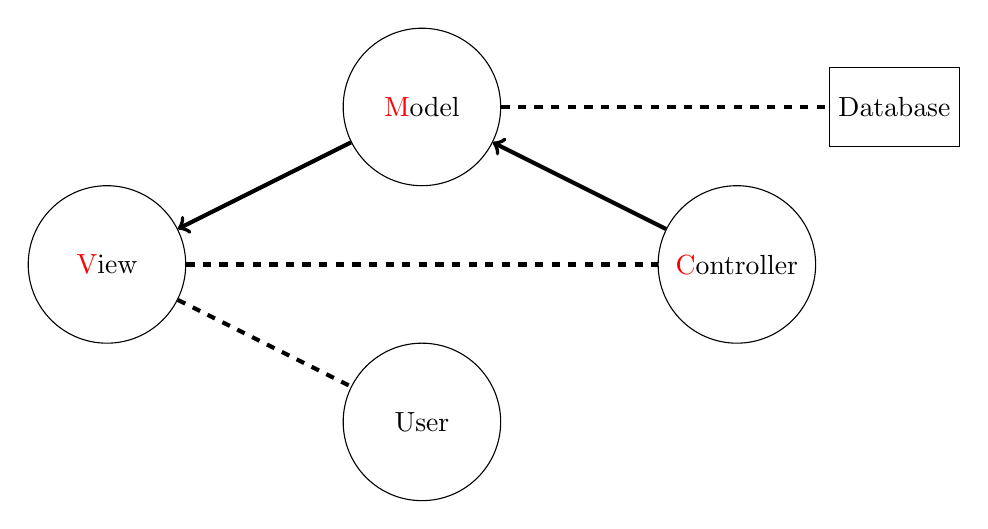
\begin{tikzpicture}
\node (DB) at (10,8) [rectangle,draw,minimum height=10mm] {Database};
\node (M) at (4,8) [circle,draw,minimum size =20mm] {\textcolor{red}{M}odel};
\node (V) at (0,6) [circle,draw,minimum size =20mm] {\textcolor{red}{V}iew};
\node (C) at (8,6) [circle,draw,minimum size =20mm] {\textcolor{red}{C}ontroller};
\node (U) at (4,4) [circle,draw,minimum size =20mm] {User};
\draw [dashed,line width=1.5pt] (M) -- (DB);

\draw [->,line width=1.5pt] (C) -- (M);
\draw [->,line width=1.5pt] (M)-- (V);
\draw [dashed,line width=1.5pt] (V) -- (U);
\draw [dashed,line width=1.5pt] (V) -- (C);
\end{tikzpicture}
\end{frame}
\begin{frame}
\frametitle{MVC的具体实现}
在不引入框架的情况下:

\begin{table}
\begin{tabular}{cc}
\toprule
\textbf{M/V/C} & \textbf{technology}\\
\midrule
V & jsp,html\\
C & servlet\\
M & java bean\\
\bottomrule
\end{tabular}
\caption{MVC的无框架实现}

\end{table}
\end{frame}
\section{servlet}
\begin{frame}
\Huge{\centerline{servlet}}
\end{frame}
\begin{frame}
\frametitle{servlet是什么}
servlet是\textcolor{red}{运行在web服务器端的java程序}。
\begin{enumerate}
\item
\textcolor{red}{封装了对HTTP请求}的处理
\item
运行\textcolor{red}{需要servlet容器}支持(比如tomcat、weblogic等)。
\end{enumerate}


servlet先于jsp产生,便是其代码组织形式是\textcolor{red}{将html代码混杂在java代码中},给web程序设计带来了很多不便,比如负责网页设计的\textcolor{red}{美工人员也需要学习java知识},从而进行页面的设计,在程序设计中,servlet产生的动态网页又需要在代码中\textcolor{red}{编写大量输出html标签的语句}。

基于以上原因,Sun公司提出了jsp技术。jsp是一种在servlet规范之上的动态网页技术,jsp文件在第一次被请求时,会被编译成servlet文件,再通过容器调用servlet进行处理。

\end{frame}
\begin{frame}[fragile]
\frametitle{servlet代码片断}
\begin{lstlisting}
1 while(enu.hasMoreElements()){
2 String attr = enu.nextElement();
3  if(attr.equals("user")){
4    user = (String)session.getAttribute("user");
5    out.print("你好,"+user+"。");
6    out.print("<form action=\"logout.jsp\"
        method=\"post\">");
7    out.print("<input type=\"submit\" 
        value=\"logout\"></form>");
8    break;
9  }
10 }
\end{lstlisting}
\end{frame}
\begin{frame}
\frametitle{servlet代码结构}

\end{frame}
\section{java bean}
\begin{frame}
\Huge{\centerline{java bean}}
\end{frame}


%------------------------------------------------

\begin{frame}
\Huge{\centerline{The End}}
\end{frame}

%---------------------------------------



%----------------------------------------------------------------------------------------

\end{document} 